\documentclass[border=10pt]{standalone}
\usepackage[svgnames]{xcolor}
\usepackage{amsmath}
\usepackage{pgfplots}
\pgfplotsset{compat=newest}
\usepackage[sfdefault]{FiraSans}
\usepackage{FiraMono}
\renewcommand*\familydefault{\sfdefault}
\begin{document}
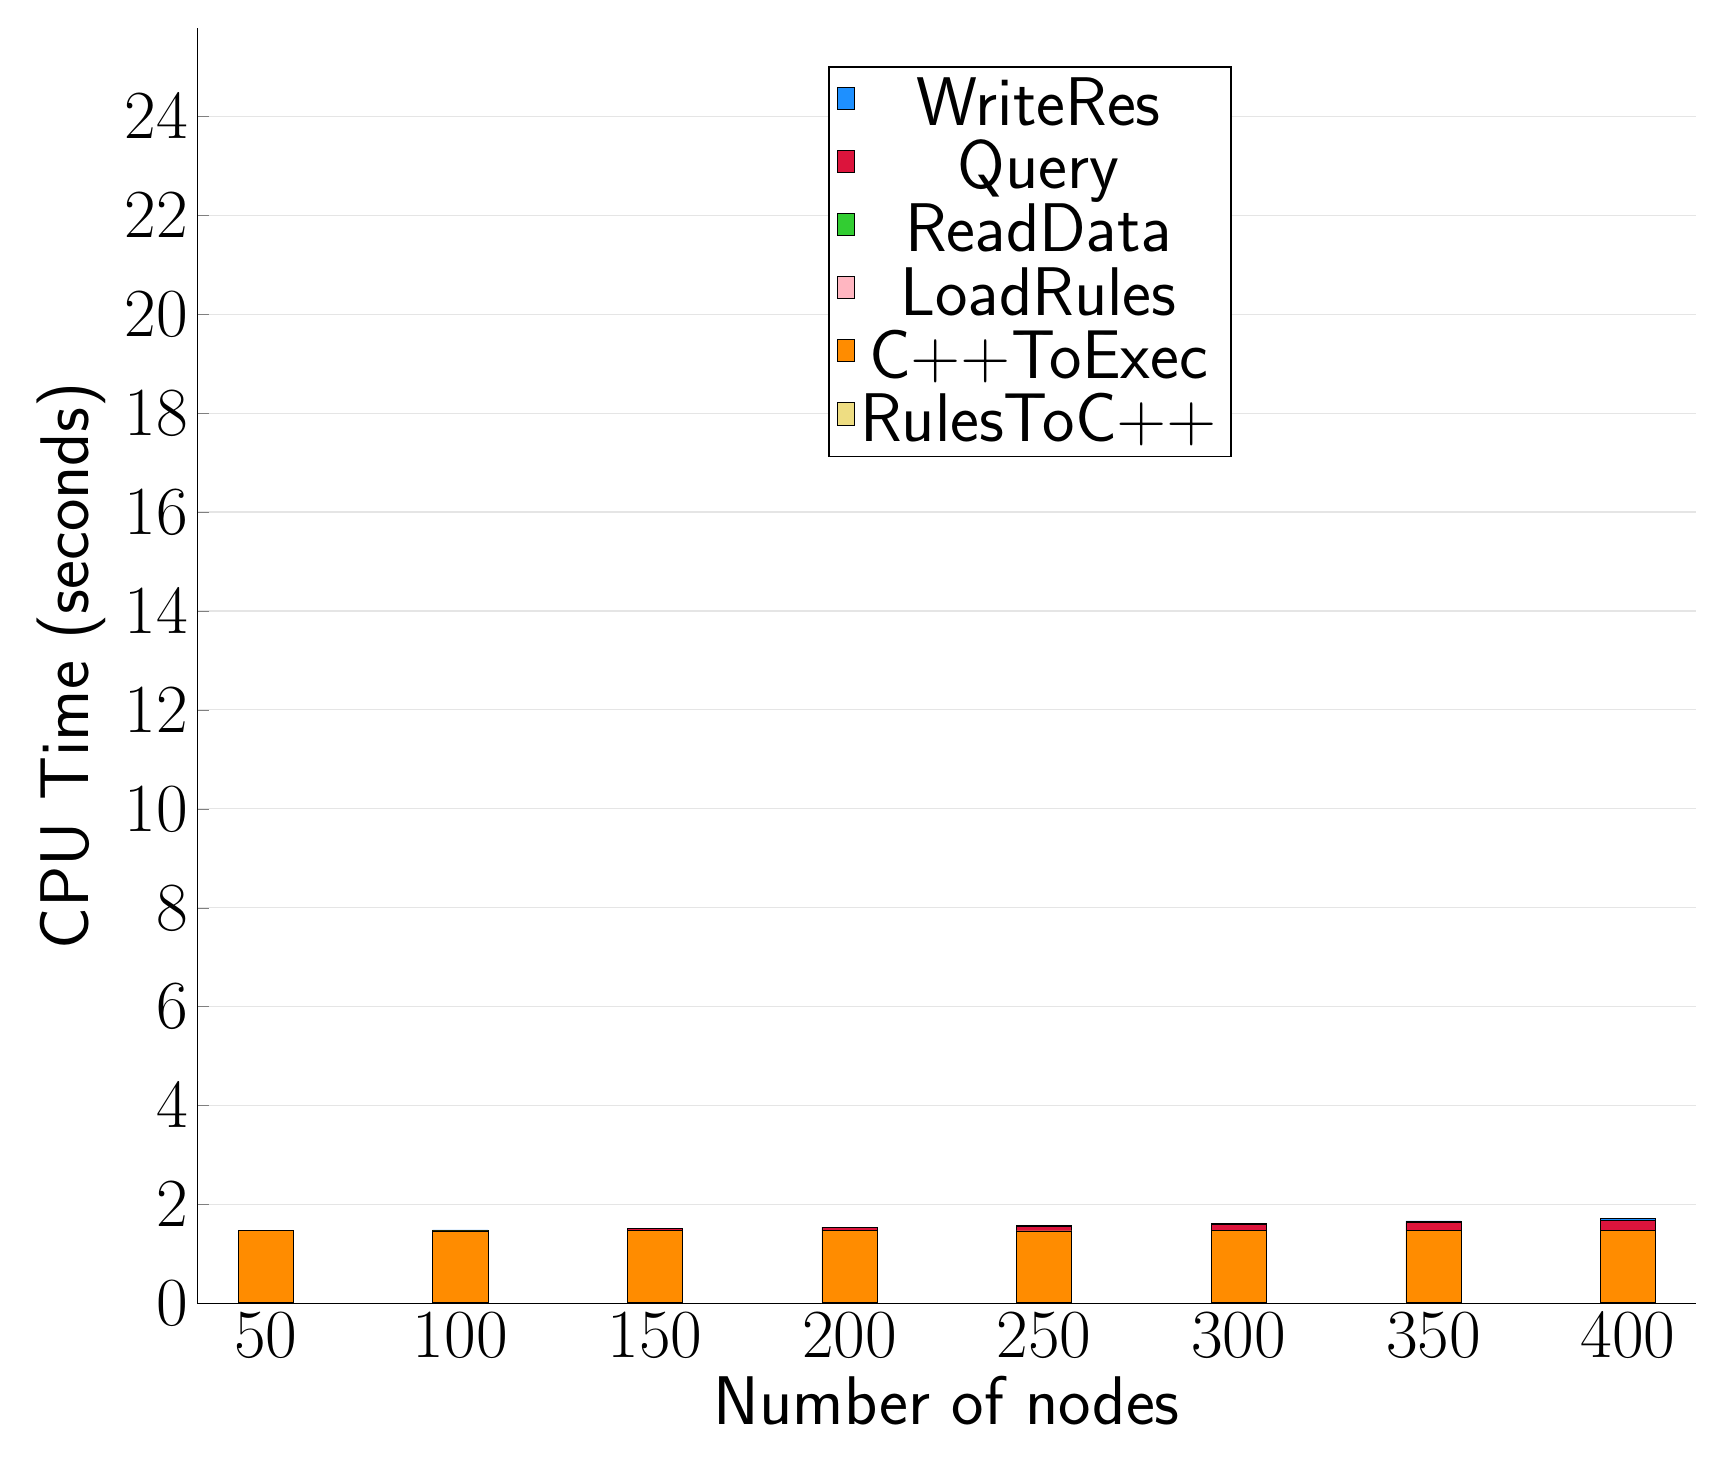
\begin{tikzpicture}
\begin{axis}[
   ybar stacked,
   width=1.7\textwidth,
   bar width=0.7cm,
   ymajorgrids, tick align=inside,
   major grid style={draw=gray!20},
   xtick=data,
   ymin=0, ymax=25.779619999999998,
   axis x line*=bottom,
   axis y line*=left,
   enlarge x limits=0.05,
   legend style={
       at={(0.69, 0.97)},
       anchor=north east,
       legend columns=1,
       font=\Huge,
   },
   ylabel={CPU Time (seconds)},
   xlabel={Number of nodes},
   label style={font=\Huge},
   tick label style={font=\Huge},
]
\addlegendimage{fill=DodgerBlue, draw=black, line width=0.2pt}
\addlegendentry{WriteRes}
\addlegendimage{fill=Crimson, draw=black, line width=0.2pt}
\addlegendentry{Query}
\addlegendimage{fill=LimeGreen, draw=black, line width=0.2pt}
\addlegendentry{ReadData}
\addlegendimage{fill=LightPink, draw=black, line width=0.2pt}
\addlegendentry{LoadRules}
\addlegendimage{fill=DarkOrange, draw=black, line width=0.2pt}
\addlegendentry{C++ToExec}
\addlegendimage{fill=LightGoldenrod, draw=black, line width=0.2pt}
\addlegendentry{RulesToC++}
\addplot +[fill=LightGoldenrod, draw=black, line width=0.2pt] coordinates {
(50, 0.031000000000000007)
(100, 0.030000000000000006)
(150, 0.030000000000000006)
(200, 0.030000000000000006)
(250, 0.030000000000000006)
(300, 0.030000000000000006)
(350, 0.030000000000000006)
(400, 0.030000000000000006)
};
\addplot +[fill=DarkOrange, draw=black, line width=0.2pt] coordinates {
(50, 1.446)
(100, 1.4389999999999998)
(150, 1.451)
(200, 1.4449999999999998)
(250, 1.4399999999999997)
(300, 1.4460000000000002)
(350, 1.4489999999999998)
(400, 1.4439999999999997)
};
\addplot +[fill=LightPink, draw=black, line width=0.2pt] coordinates {
(50, 2.5300000000000002e-05)
(100, 0.0)
(150, 1.11e-05)
(200, 1.01e-05)
(250, 1.09e-05)
(300, 1.09e-05)
(350, 1.1e-05)
(400, 1.11e-05)
};
\addplot +[fill=LimeGreen, draw=black, line width=0.2pt] coordinates {
(50, 0.0004142)
(100, 0.0005162)
(150, 0.0006143)
(200, 0.0007325)
(250, 0.0008121000000000002)
(300, 0.0008624000000000001)
(350, 0.0010308)
(400, 0.0011068999999999999)
};
\addplot +[fill=Crimson, draw=black, line width=0.2pt] coordinates {
(50, 0.0043143)
(100, 0.0159942)
(150, 0.03501230000000001)
(200, 0.0576405)
(250, 0.08530890000000001)
(300, 0.11729890000000001)
(350, 0.1592501)
(400, 0.20581960000000002)
};
\addplot +[fill=DodgerBlue, draw=black, line width=0.2pt] coordinates {
(50, 0.0013817)
(100, 0.0039406)
(150, 0.0074017)
(200, 0.011368800000000002)
(250, 0.017483199999999997)
(300, 0.025026399999999997)
(350, 0.0343169)
(400, 0.045253400000000006)
};
\end{axis}
\end{tikzpicture}

\end{document}
